\renewcommand{\lecturetitle}{Motivation}
\renewcommand{\lecturetime}{Week 9, Video 1}
\section{\lecturetitle}
%-------------------------------------------------
%-------------------------------------------------

%-----------------------------------------------------------------------
\myframe{Motivation for Neural Architecture Search}{

	\centering
	\begin{itemize}
	  \item Performance improvements on various tasks due to novel architectures
%	  Designing neural network architectures is hard, requiring lots of human efforts
	  \item Can we automate this design process, potentially discovering new components/topologies?
	\end{itemize}

\bigskip
\bigskip
		
	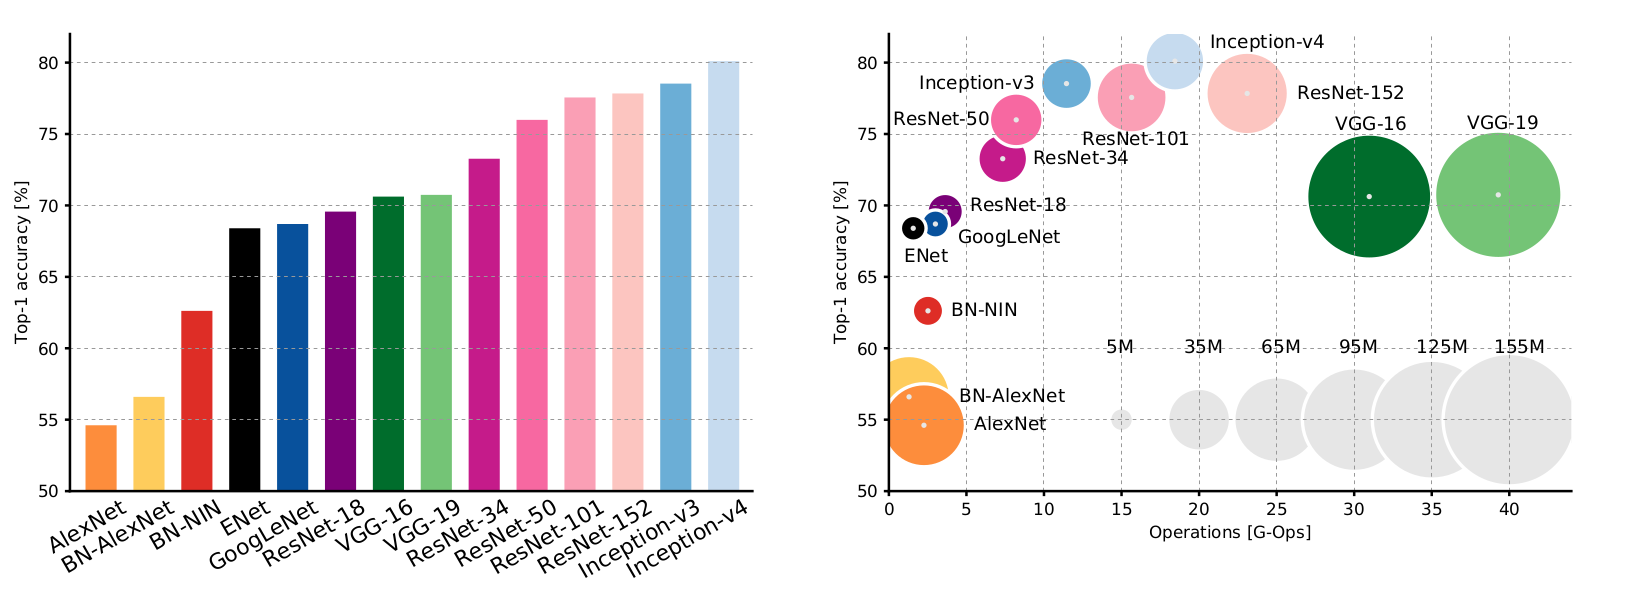
\includegraphics[width=.9\textwidth]{images/architectures_perf2.png}\\
	\href{https://arxiv.org/pdf/1605.07678.pdf}{\lit{Canziani et al. 2017}}

}
%-----------------------------------------------------------------------

%----------------------------------------------------------------------
\myframetop{Motivation for Neural Architecture Search}{

\begin{itemize}
	\item Manual design of architectures is \alert{time consuming}
	\item Complex state-of-the-art architectures are a result of \alert{years of trial} and errors by experts.
\end{itemize}

\centering
%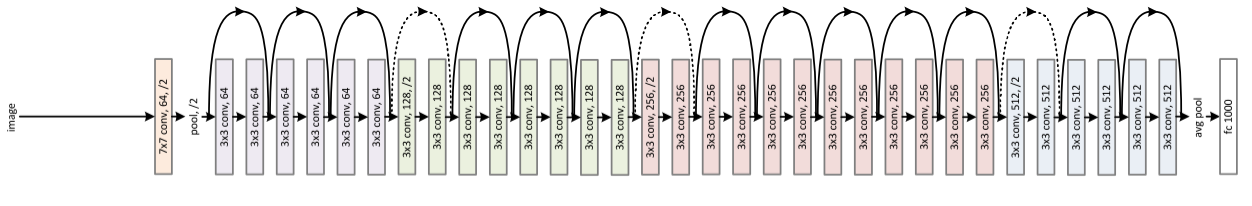
\includegraphics[width=0.8\textwidth]{images/resnet.png}\\
%\footnotesize{34-layer ResNet \href{https://www.cv-foundation.org/openaccess/content_cvpr_2016/papers/He_Deep_Residual_Learning_CVPR_2016_paper.pdf}{\lit{He et al. 2015}}}

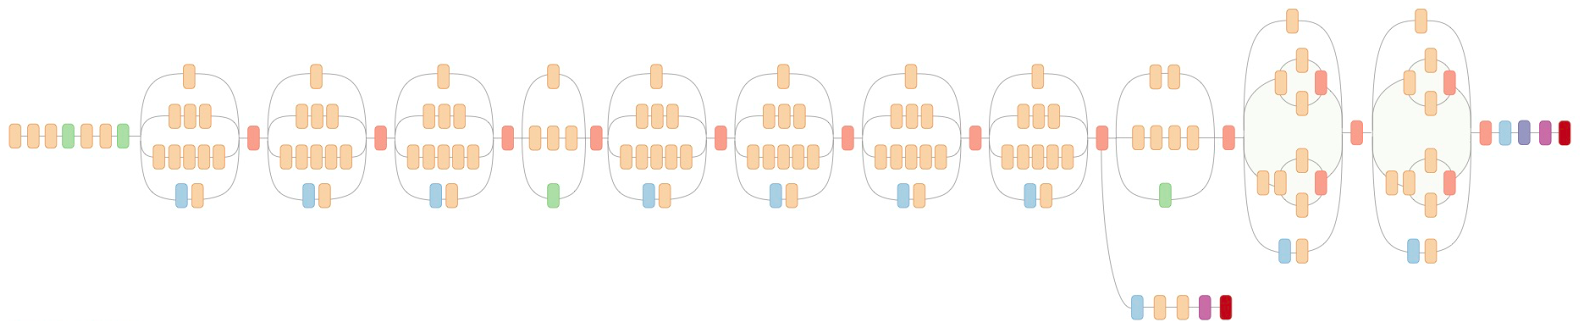
\includegraphics[width=0.8\textwidth]{images/inception.png}\\
\footnotesize{Inception-v3 \href{https://arxiv.org/abs/1512.00567}{\lit{Szegedy et al. 2016}}}

}
%-----------------------------------------------------------------------

%----------------------------------------------------------------------
\myframetop{Motivation for Neural Architecture Search}{

\begin{itemize}
	\item Manual design of architectures is \alert{time consuming}
	\item Complex state-of-the-art architectures are a result of \alert{years of trial} and errors by experts.
	\begin{itemize}
		\item[-] Main pattern: Repeated blocks with same structure (topology).
	\end{itemize}
\end{itemize}
\bigskip

\begin{columns}

\column{0.5\textwidth}
\centering
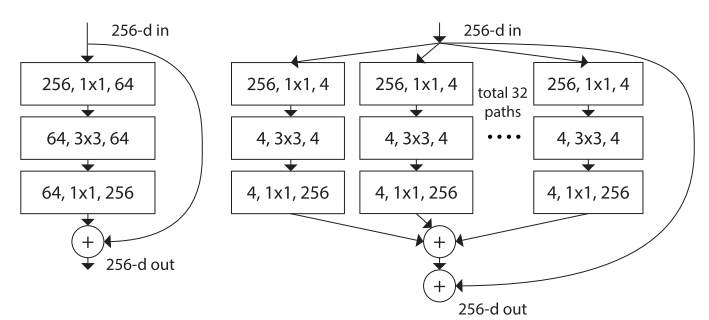
\includegraphics[width=.85\textwidth]{images/resnet_block.png}\\
\footnotesize{ResNet/ResNeXt blocks\\ \lit{\href{https://arxiv.org/abs/1603.05027}{He et al. 2016}; \href{https://arxiv.org/abs/1611.05431}{Xie et al. 2016}}}

\column{0.5\textwidth}
\centering
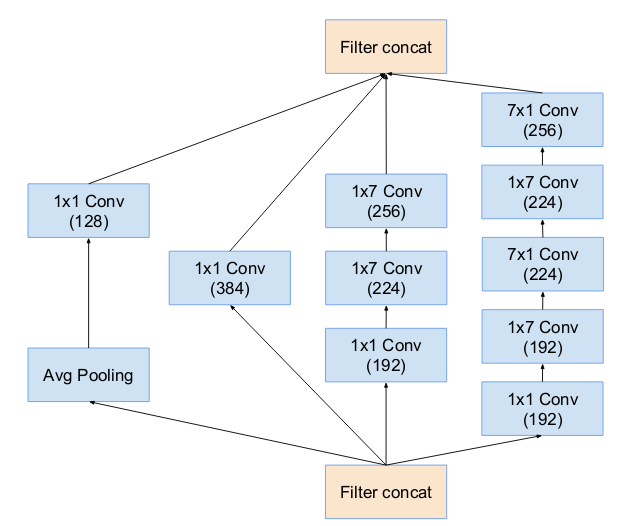
\includegraphics[width=0.4\textwidth]{images/inception_1.png}
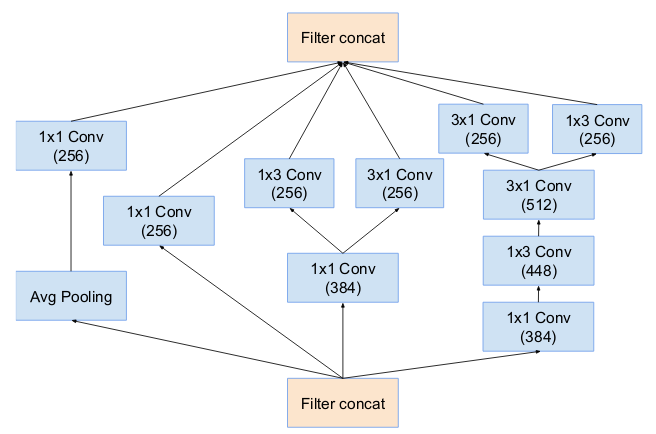
\includegraphics[width=0.4\textwidth]{images/inception_2.png}\\
\footnotesize{Inception-v4 blocks \href{https://arxiv.org/abs/1602.07261}{\lit{Szegedy et al. 2017}}}

\end{columns}
}
%-----------------------------------------------------------------------

%-----------------------------------------------------------------------
\myframe{Meta-Remark: Issues in NAS Research \& Evaluations}{

	\begin{columns}[T]
	\column{0.50\textwidth}
	\begin{itemize}
	  \item For benchmarks used in almost all NAS papers:
	  \myit{
	  	\item[-] \alert{Training pipeline matters much more than neural architecture}
	  }
\bigskip
	  \onslide<2->{
		  \item The final benchmark results reported in different papers are typically \alert{incomparable}
		  \myit{
		  	\item[-] \alert{Different training code\\ (often unavailable)}
		  	\item[-] \alert{Different search spaces}
		  	\item[-] Different evaluation schemes
		  }
	  }
\bigskip
	  \onslide<3->{
	  	\item[$\rightarrow$] We will emphasize \alert{concepts}, not published performance numbers
	  }
	\end{itemize}
		
	\column{0.02\textwidth}
	\column{0.48\textwidth}
		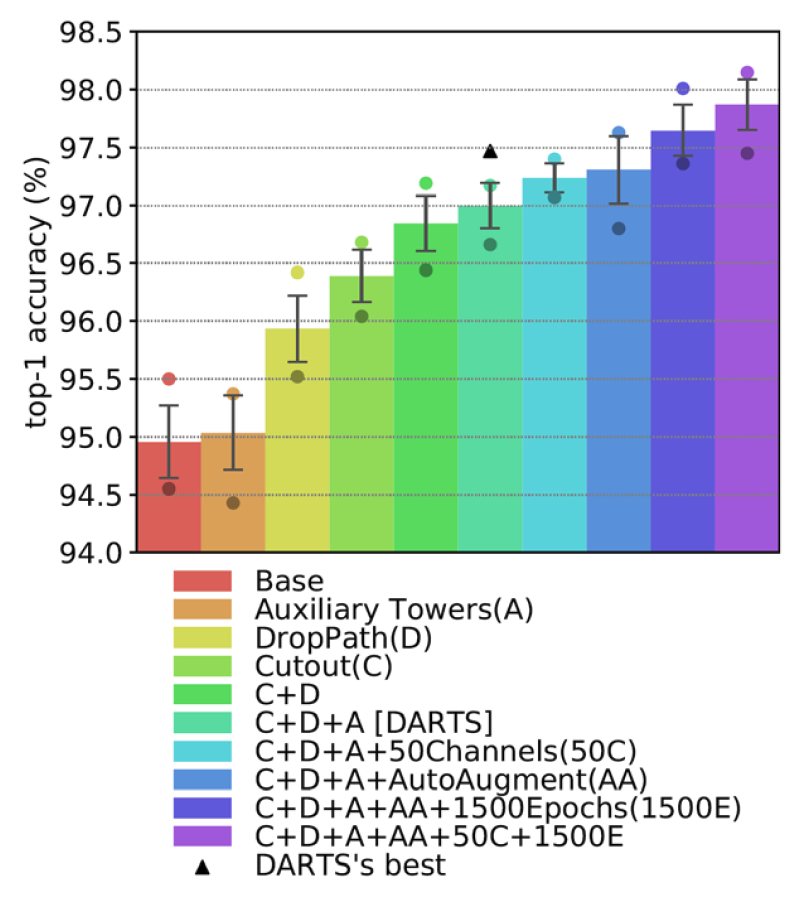
\includegraphics[width=.8\textwidth]{images/nas-eval-is-frustatingly-hard}\\
		\centering
		\href{https://openreview.net/forum?id=HygrdpVKvr}{\lit{Yang et al., ICLR 2020}}
	\end{columns}
	
}
%-----------------------------------------------------------------------

%-----------------------------------------------------------------------
\myframe{Meta-Remark: Building a Scientific Community for NAS}{

	\myit{
	  \item \alert{Benchmarks}
	  \myit{
	  	\item[-] NAS-Bench-101 \href{https://arxiv.org/pdf/1902.09635.pdf}{\lit{Ying et al, ICML 2019}}
	  	\item[-] NAS-Bench-201 \href{https://openreview.net/forum?id=HJxyZkBKDr}{\lit{Dong et al, ICML 2020}}
	  	\item[-] NAS-Bench-1Shot1 \href{https://openreview.net/forum?id=SJx9ngStPH}{\lit{Zela et al, ICLR 2020}}
	  }
\medskip
\pause
	  \item \alert{Best Practice Checklist} for Scientific Research in NAS\\ \href{https://arxiv.org/abs/1909.02453}{\lit{Lindauer \& Hutter, arXiv 2019}}
\medskip
\pause
	  \item \alert{Unifying open-source implementation} of modern NAS algorithms \\ \href{https://openreview.net/forum?id=SJx9ngStPH}{\lit{Zela et al, ICLR 2020}}
	  \myit{
	  	\item[-] Finally enables empirical comparisons without confounding factors	  	
	  }
\medskip
\pause
	  \item \alert{\href{https://sites.google.com/view/nas2020}{First NAS workshop}} at ICLR 2020
	  
	}
}
%-----------------------------------------------------------------------

%----------------------------------------------------------------------
%\myframe{Brief history and early approaches}{
%\centering
%
%\begin{itemize}
%\footnotesize{
%	\item The very first works (to the best of our knowledge):
%	\begin{itemize}
%		\item Self Organizing Neural Networks \href{https://papers.nips.cc/paper/149-self-organizing-neural-networks-for-the-identification-problem}{\lit{Tenorio and Lee, NeurIPS 1988}}
%		\item The Cascade-Correlation Learning Architecture \href{https://papers.nips.cc/paper/207-the-cascade-correlation-learning-architecture}{\lit{Fahlman and Lebiere, NeurIPS 1989}}
%	\end{itemize}
%}
%\end{itemize}
%
%\pause
%
%\begin{columns}
%\column{0.57\textwidth}
%\centering
%
%\vspace{-2cm}
%\begin{itemize}
%\footnotesize{
%	\item \alert{Neuroevolution} (already since the 1990s)
%	\begin{itemize}
%		\item Some authors used evolutionary algorithms to optimize the
%		architecture and backpropagation for weights \lit{\href{https://www.complex-systems.com/abstracts/v04_i04_a06/}{Kitano 1990}}
%		\item In neuroevolution both architecture and weights are optimized with
%		evolutionary methods \lit{\href{http://nn.cs.utexas.edu/downloads/papers/stanley.ec02.pdf}{Stanley and Miikkulainen, 2002}; \href{https://link.springer.com/article/10.1007/s12065-007-0002-4}{Floreano et al. 2008}}	
%	\end{itemize}	
%}
%\end{itemize}
%
%\column{0.4\textwidth}
%\centering
%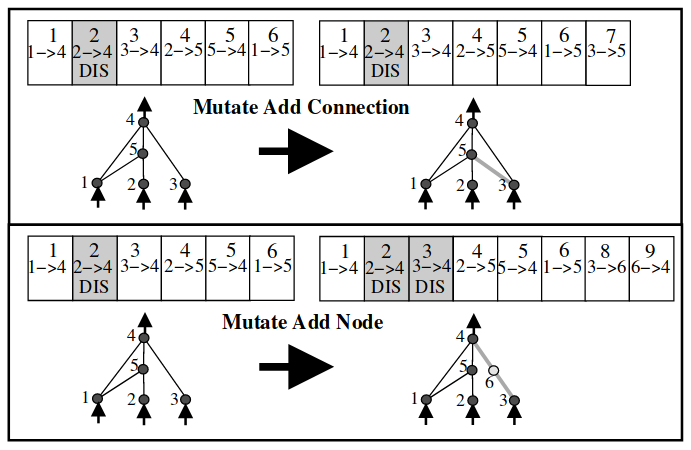
\includegraphics[width=0.6\textwidth]{images/neat.png}\\
%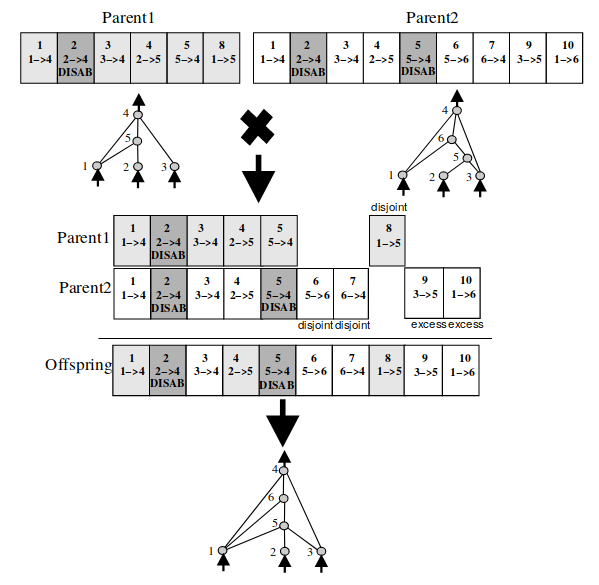
\includegraphics[width=0.6\textwidth]{images/neat_2.png}
%\end{columns}
%
%}
%-----------------------------------------------------------------------

%----------------------------------------------------------------------
%\myframe{Brief history and early approaches}{
%\centering
%
%\begin{itemize}
%\footnotesize{
%	\item \alert{Bayesian optimization (BO)}
%	\begin{itemize}
%		\item Encode the architecture as a categorical space
%		\begin{itemize}
%			\item[-] i.e. optimize number of layers, number of filters, kernel width, etc.		
%		\end{itemize}
%		\item Use BO to search in this categorical space \lit{\href{http://proceedings.mlr.press/v28/bergstra13.pdf}{Bergstra et al. 2013}, \href{https://ml.informatik.uni-freiburg.de/papers/15-IJCAI-Extrapolation_of_Learning_Curves.pdf}{Domhan et al. 2015}, \href{https://ml.informatik.uni-freiburg.de/papers/16-AUTOML-AutoNet.pdf}{Mendoza et al. 2015}, \href{https://arxiv.org/abs/1807.06906}{Zela et al. 2018}}
%	\end{itemize}
%}
%	\pause
%	\item Reinforcement Learning \& Evolution for NAS \lit{\href{https://arxiv.org/abs/1611.02167}{Baker et al. 2016}, \href{https://arxiv.org/abs/1611.01578}{Zoph and Le 2017}, \href{https://arxiv.org/abs/1707.07012}{Zoph et al. 2018}, \href{https://arxiv.org/abs/1703.01041}{Real et al. 2017}, \href{https://arxiv.org/abs/1802.01548}{Real et al. 2018}}
%
%	\pause
%	\item \alert{Recent work aims for efficiency}
%		\begin{itemize}
%			\begin{footnotesize}
%			\item Weight sharing \lit{Pham et al,’18; Bender et al, ’18; Liu et al, ‘19; Xie et al. ’19; Cai et al. ’19, Zhang et al. ’19}
%			\item Network morphisms \lit{Chen et al, ’16; Cai et al, ’17 \& ‘18; Elsken et al, ’17 \& 18}
%			\item Multi-fidelity optimization \lit{Klein et al, ‘16; Li et al, ‘18; Falkner et al, ‘18}
%			\end{footnotesize}
%		\end{itemize}
%	\end{itemize}
%
%TODO: add hrefs to recent work
%}
%-----------------------------------------------------------------------

%-----------------------------------------------------------------------
\myframe{NAS components \litw{\href{http://jmlr.org/papers/v20/18-598.html}{Elsken et al. 2019}}}{

\centering
%\hspace{1cm}
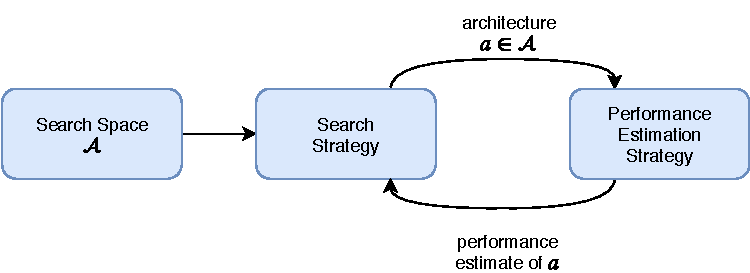
\includegraphics[width=0.9\textwidth]{images/NAS_diagram.pdf}

\begin{itemize}
	\item \alert{Search Space:} the types of architectures we consider; micro, macro, hierarchical, etc.
	\item \alert{Search Strategy:} RL, ES, BO, gradient-based, etc.
	\item \alert{Performance Estimation Strategy:} validation performance, \\ lower fidelity estimates, one-shot model performance, etc.
\end{itemize}

}
%----------------------------------------------------------------------


%----------------------------------------------------------------------
\myframe{Questions to Answer for Yourself / Discuss with Friends}{

	\myit{
		\item Repetition:\\ \alert{For the most common NAS search space, how important is the NAS component
		compared to the importance of the training pipeline used?}\medskip
\medskip
%		\item Repetition:\\ \alert{How are the weights optimized in neuroevolution?}
		\item Repetition:\\ \alert{List three major components of NAS methods.}
\medskip
		\item Discussion:\\ \alert{Which problems would you like to apply NAS to?}
	}	 
}
%-----------------------------------------------